In this chapter we explore some consequences of a basic mathematical fact called the \textbf{Pigeonhole Principle}. Although the statement itself is very elementary, the various consequences and results that one can obtain as a consequence of this basic fact are very deep and surprising. In the first section we will explore the pigeonhole principle's application in the finite case and the infinite case.

\section{The Pigeonhole Principle}
The most basic statement of the pigeonhole principle seems so obvious that it may not be apparent that it actually requires proof.

\begin{proposition}
Suppose I have $n$ pigeons and $m$ holes, with $n > m$. No matter how I put the pigeons into the holes, I will have a hole that contains at least 2 pigeons.
\end{proposition}
\begin{proof}
Suppose this is not true. Then there is a way to place the m pigeons such that each hole has less than or equal to one pigeon. Then the total number of pigeons would be less than or equal to $m \cdot 1 = m$ pigeons. But there are $n > m$ pigeons. This is a contradiction and the statement follows.
\end{proof}

We can more formally state the pigeonhole principle as follows: suppose $n > m$. Then for any function $f:\{1, \dots, n\} \to \{1, \dots, m\}$ there exists a $k$ between $1$ and $m$ inclusive such that $|f^{-1}(k)| > 1$.

\begin{example}
Here is an illustration of the pigeonhole principle when $n = 4$ and $m = 3$. In the following diagram, the ``holes" are the boxes and the ``pigeons'' are the blue balls.

\begin{centering}
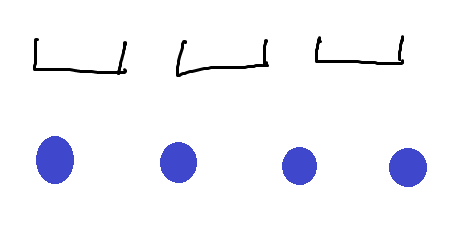
\includegraphics[width=3in]{Ch9/pigeonholeex11}
\end{centering}

Here is an example of balls being put into the boxes.

\begin{centering}
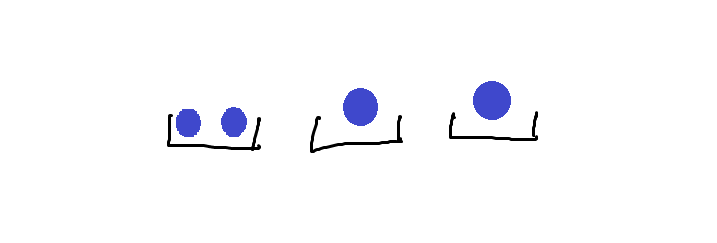
\includegraphics[width=5in]{Ch9/pigeonholeex12}
\end{centering}

\end{example}

With this principle, it is possible to prove some facts that don't seem like they follow from this simple proposition.

\begin{example}
Suppose that we are at a party with $n$ people. At this party, people shake hands with one another. Then no matter how they shake hands, at least two people shook hands with the same number of people. The reasoning is as follows. Consider the possible values for hands shaken for each individual. Normally, this ranges from $0$ (no hands shaken) to $n-1$ (hands shaken with everyone else). If we consider these the holes, the pigeonhole principle does not immediately guarantee that 2 people will have shaken the same number of hands. However, we observe that if someone has shaken hands with $n-1$ people, they've shaken hands with everyone else, so that no one will have shaken hands with $0$ people. The same logic applies once someone has shaken $0$ hands. Hence we can use the pigeonhole principle to conclude that two people have shaken the same number of hands.
\end{example}



\section{Ramsey's Theorem}

\subsection{Infinite Ramsey Implies Finite Ramsey}
In this section we prove the observation that the Infinite Ramsey Theorem implies the Finite Ramsey Theorem. The idea we will use is a common argument called a ``subsequence argument'': passing (many times) to subsequences we will find a sequence of complete (but finite graphs) each of which avoid a coloring we are avoiding and are related to each other. In this way we find a coloring of the complete graph on $\mathbb{N}$ which avoids this coloring as well.

\begin{theorem}
Assume that the following theorem is true: If $K_\mathbb{N}$ is edge-colored with two colors, then there exists an infinite subset $S \subset \mathbb{N}$ such that the subgraph $K_S$ is monochromatic. Then the following theorem is true. For all $n \in \mathbb{N}$ there exists $N(n) \in \mathbb{N}$ such that if $K_N$ is edge-colored red or blue then $K_N$ contains a monochromatic $K_n$.
\end{theorem}

\begin{proof}
We will assume the contrary. Then we will be done if we construct a coloring of $K_N$ which does not contain a monochromatic infinite $K_S$.

Suppose now this is true. Then there exists $n \in \mathbb{N}$ such that for all $N \in \mathbb{N}$ there is a edge-coloring $J_N$ of $K_N$ which avoids a monochromatic $K_n$. To make choices consistent suppose we label $K_N$'s vertices $\{1, 2, \dots, N\}$. Now we find a ``nice'' subsequence of these colors as follows:

\begin{enumerate}
	\item First enumerate the set of edge pairs $\{a, b\} \subset \mathbb{N}$ as $e_i$, which is possible because this set is countable. 
	\item For $e_1$, for each graph where this edge exists, we can find a subsequence $J_{i_1}, J_{i_2}, \dots$ where in each coloring where applicable the edge $e_i$ is colored the same. (We can include the colorings where $e_i$ does not exist, since there are only finitely many of these).
	\item Do the same inductively for $e_2, e_3, \dots$.
\end{enumerate}
In the end we have a subsequence of colorings
\[J_{j_1}, J_{j_2}, \dots\]
with the following properties:
\begin{itemize}
	\item The $J_{j_k}$ avoid any monochromatic $K_n$,
	\item For any edge $e_i = \{a, b\}$ every $J_{j_k}$ colors $e_i$ the same color.
\end{itemize}

We can use this to define a coloring of $K_\mathbb{N}$ as follows. For each edge $e_i$ we color this edge by the unique color that is assigned to it by the $J_{j_k}$. It is clear that this coloring avoids a monochromatic $K_n$. Indeed, we observe that if such a coloring on the edges between the vertices $m_1, \dots, m_n$ was monochromatic then we can find some $j_k > \max(m_1, \dots, m_n)$ and we observe that this cannot be monochromatic. So we are done now since a monochromatic $K_S$ where $S$ is infinite necessarily contains a monochromatic $K_n$.
\end{proof}
